\chapter{Caractéristiques fonctionnelles}

\section{Définition des acteurs}

Le Paragraphe suivant explicite les divers acteurs du projet et leurs rôles :
\begin{itemize}
	\item Formateurs : sera le Maitre du Jeux personnes qui pourra choisir les thèmes des carte a aborder lors de la séance de jeu et pourra aussi crée a près les cartes en rajoutant au paquet via un document fournies.
	\item Stagiaire : sera les Joueur qui pourront jouer au jeu lors de la séance de jeu. 
\end{itemize}

\section{Diagramme pieuvre}

%:-+-+-+- 
\begin{figure} [!ht]
	\centering
	% Racine en Bas, développement vers le haut
	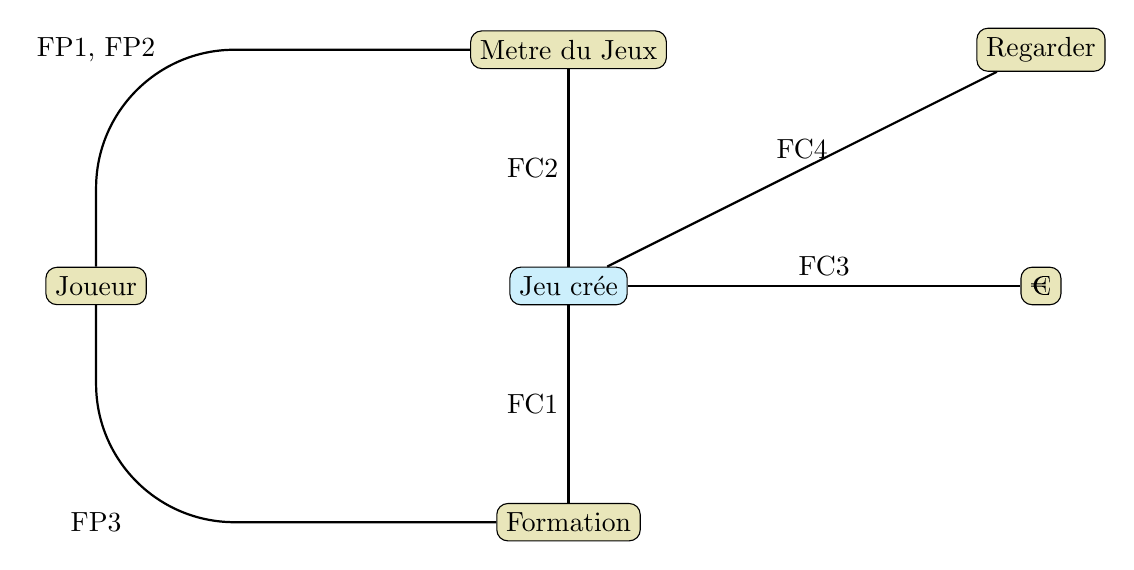
\begin{tikzpicture}[xscale=1,yscale=1]
		% Styles (MODIFIABLES)
		\tikzstyle{lienIndiecret}=[-,>=latex,thick,rounded corners=50pt]
		\tikzstyle{lienDiecret}=[-,>=latex,thick]
		\tikzstyle{but}=[fill=cyan!20,draw,rounded corners=4pt]
		\tikzstyle{app}=[fill=olive!20,draw,rounded corners=4pt]
		
		\tikzstyle{etiquette}=[midway,fill=white,draw]
		% Dimensions (MODIFIABLES)
		\def\DistanceInterNiveaux{3}
		\def\DistanceInterFeuilles{2}
		% Dimensions calculées (NON MODIFIABLES)
		\def\NiveauA{(1)*\DistanceInterNiveaux}
		\def\NiveauB{(0)*\DistanceInterNiveaux}		
		\def\NiveauC{(-1)*\DistanceInterNiveaux}
		
		\def\InterFeuilles{(1)*\DistanceInterFeuilles}
		% Noeuds (MODIFIABLES : Styles et Coefficients d'InterFeuilles)
		%\node[tete] (Ta) at ({(-2)*\InterFeuilles},{\NiveauA}) {A sui rend-il service ?};
		\node[app] (Mj) at ({(0)*\InterFeuilles},{\NiveauA}) {Metre du Jeux};
		\node[app] (R) at ({(3)*\InterFeuilles},{\NiveauA}) {Regarder};
		\node[app] (S) at ({(3)*\InterFeuilles},{\NiveauB}) {€};
		\node[but] (but) at ({(0)*\InterFeuilles},{\NiveauB}) {Jeu crée};
		\node[app] (J) at ({(-3)*\InterFeuilles},{\NiveauB}) {Joueur};
		\node[app] (F) at ({(0)*\InterFeuilles},{\NiveauC}) {Formation};
		
		
		% Arcs (MODIFIABLES : Styles)
		%\draw[corne] (App.north)-|(sTa) node[midway,fill=white]{oui};
		%\draw[lienbut] (App.east) --  ({(1.5)*\InterFeuilles},{\NiveauC}) -- ({(1.5)*\InterFeuilles},{\NiveauG}) -- (ButsT.east) ;
		\draw[lienIndiecret] (Mj) -| (J) node[midway] {FP1, FP2};
		\draw[lienIndiecret] (J) |- (F) node[midway] {FP3};
		\draw[lienDiecret] (but) -- (F) node[midway,left] {FC1};
		\draw[lienDiecret] (but) -- (Mj) node[midway,left] {FC2};
		\draw[lienDiecret] (but) -- (S) node[midway,above] {FC3};
		\draw[lienDiecret] (but) -- (R) node[midway,above] {FC4 };
		
		
	\end{tikzpicture}
	\caption{Diagramme pieuvre de l'analyse fonctionnelle}
\end{figure}
%:-+-+-+-+- Fin

Ce document permet d'organiser les Fonctions Principales FP, les Fonction Contrainte FC, les Fonction Technique et Pratique FTP.\\
\begin{center}
	\rotatebox{90}{
		\begin{tabular}{|c|c|c|c|c|c|}
			\hline
			Types & ordre &                               intituler                                &  Priori-  &                   &                              \\
			      &       &                                                                        &   taire   &     Critères      &           Niveaux            \\
			      &       &                                                                        & du client &                   &                              \\ \hline
			 FP   &   1   &    Permettre lire la question entre le Maitre du Jeu et les Joueur.    &    ?1?    & - Quater du texte &     - écrit en français      \\ \hline
			 FP   &   2   & Permettre répondre à la question entre les Joueur et le Maitre du Jeu. &    ?1?    &   - thème connu   &      - par les joueurs       \\ \hline
			 FP   &   3   &        Permettre être en lien entre le Joueur et ca Formation.         &    ?1?    &      - thème      &       - lien en module       \\ \hline
			 FC   &   1   &                   Doit être adapter a la Formation.                    &     1     &     - cuiter      & - ludique et lien formation  \\ \hline
			 FC   &   2   &            Doit s'utiliser facilement par le Maitre du Jeu.            &     2     &  - type de réglé  &     - Simple et intuitif     \\ \hline
			 FC   &   3   &             Doit avoir un prix de fabrication raisonnable.             &    ?4?    &      - Prix       & - Compatible a tout le monde \\ \hline
			 FC   &   4   &                          Doit plaire à l'œil.                          &    ?5?    &      - Forme      &       - rectangulaire        \\
			      &       &                                                                        &           &     - Couleur     &           - sobre            \\ \hline
			 FTP  &   1   &                       Doit se ranger facilement.                       &     3     &                   &                              \\ \hline
			 FTP  &   2   &                    Doit se transporter facilement.                     &     3     &                   &                              \\ \hline
			%FTP  &   3   &                      Doit être écrit en français.                      &     4     &                   &                              \\ \hline
			 FTP  &   4   &                       Doit être un jeux a thème.                       &    ?5?    &                   &                              \\ \hline
			 FTP  &   5   &           Doit avoir un Nombre de carte pour fini la partie.           &    ?5?    &                   &                              \\ \hline
			 FTP  &   6   &             Doit avoir un Nombre de carte Minimum 50-100.              &    ?5?    &                   &                              \\ \hline
			 FTP  &   7   &                 Doit être un jeux de carte de Hasard.                  &    ?5?    &                   &                              \\ \hline
			 FTP  &   8   &                   Doit être fini entre 15-20 minute.                   &    ?5?    &                   &                              \\ \hline
		\end{tabular}
	}
\end{center}